\begin{frame}
\frametitle{Системные вызовы}
\begin{itemize}
  \item Системные вызовы - это механизм взаимодействия непривелигерованного кода
  (пользовательских приложений) и привелигированного кода (ядра)
  \begin{itemize}
    \item open/close, read/write, fork, exec и др. требуют обращения к ядру ОС.
  \end{itemize}
  \item Системный вызов осуществляет контролируемое повышение привелегий:
  \begin{itemize}
    \item нельзя дать произвольному коду выполняться в привелигированном режиме;
    \item при системном вызове вызывается определенная функция ядра ОС;
    \item функция ОС должна параноидально проверять все аргументы системного
    вызова на корректность.
  \end{itemize}
\end{itemize}
\end{frame}

\begin{frame}
\frametitle{Организация системных вызовов}
\begin{center}
  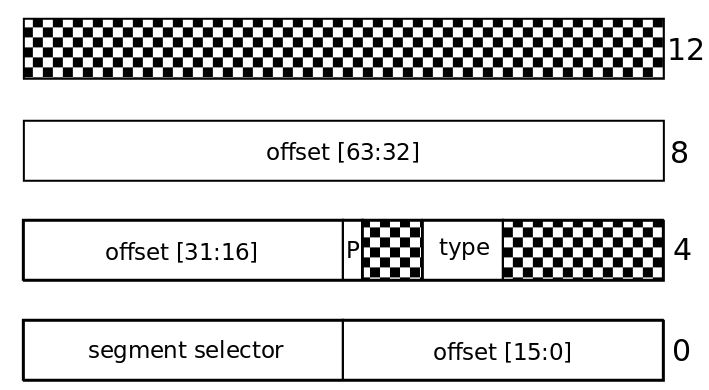
\includegraphics[width=.7\linewidth]{idt.png}
\end{center}
\begin{itemize}
  \item Типичный способ организации системного вызова - прерывания:
  \begin{itemize}
    \item например, в x86 можно использовать запись IDT с DPL равным 3;
    \item на практике используют специальные инструкции syscall/sysenter потому
    что они работают быстрее.
  \end{itemize}
\end{itemize}
\end{frame}

\begin{frame}
\frametitle{Передача аргументов и возврат значений}
\begin{itemize}
  \item При системном вызове типичным способом передачи аргументов и возврата
  значений являются регистры:
  \begin{itemize}
    \item например, в Linux Kernel используется следующая конвенция:
    \begin{itemize}
      \item регистр RAX соедржит номер системного вызова;
      \item регистры RDI, RSI, RDX, R10, R8, R9 содержат аргументы;
      \item результат возвращается в регистре RAX.
    \end{itemize}
  \end{itemize}
\end{itemize}
\end{frame}

\begin{frame}[fragile]
\frametitle{Пример: linux hello world}
\lstinputlisting{src/hello.S}
\end{frame}

\begin{frame}
\frametitle{Стек системного вызова}
\begin{itemize}
  \item Ядро оперирует данными всех приложений - не хочется, чтобы эти данные
  "утекали" в пространство пользователя:
  \begin{itemize}
    \item если обработчик системного вызова будет использовать стек приложения
    после возврата данные могут "утеч" в пространство пользователя;
    \item соответсвенно обработчик должен использовать другой стек, либо стек
    нужно "занулять" на выходе из системного вызова.
  \end{itemize}
\end{itemize}
\end{frame}

\begin{frame}
\frametitle{Стек системного вызова}
\begin{itemize}
  \item Ядро не знает размер стека пользовательского приложения:
  \begin{itemize}
    \item приложение могло использовать почти весь свой стек, и не оставить
    ничего ядру - мы не знаем, что приложение делало до системного вызова;
    \item т. е. для обработчика системного вызова, в конечном итоге, требуется
    свой стек, который выделяется ядром.
  \end{itemize}
\end{itemize}
\end{frame}

\begin{frame}
\frametitle{Task-State Segment (TSS)}
\begin{itemize}
  \item Task-State Segment - область памяти, в которой хранится информация о
  состоянии потока исполнения:
  \begin{itemize}
    \item в 32 битном x86 могла использоваться для аппаратного переключения
    контекста;
    \item в 64 битном x86 хранит указатель стека привилегированного режима
    \begin{itemize}
      \item при системном вызове/прерывании CPU загружает в RSP значения
      записанные в TSS перед вызовом обработчика.
    \end{itemize}
    \item структура TSS описана в разделе 7.7 Task Management in 64-bit Mode
    документации Intel.
  \end{itemize}
\end{itemize}
\end{frame}

\begin{frame}
\frametitle{Использование TSS}
\begin{itemize}
  \item Для использования TSS нужно выполнить две вещи:
  \begin{itemize}
    \item завести дескриптор в GDT описывающий TSS (формат дескриптора приведен
    в разделе 7.2.3 TSS Descriptor in 64-bit mode документации Intel);
    \item загрузить селектор этой записи в Task Register используя инструкцию
    LTR (раздел 7.2.4 Task Register документации Intel).
  \end{itemize}
\end{itemize}
\end{frame}

\begin{frame}
\frametitle{Соотношение TSS и потоков}
\begin{itemize}
  \item Похоже, изначально предполагалось использовать свою TSS для каждого
  потока
  \begin{itemize}
    \item гораздо проще завести по одной TSS на ядро, загрузить Task Register
    один раз для каждого ядра и при переключении потоков изменять
    непосредственно TSS;
    \item таким образом получается, что у каждого потока есть два стека: стек
    пространства ядра и стек пространcтва пользователя (если поток вообще
    работает в пространстве пользователя).
  \end{itemize}
\end{itemize}
\end{frame}
